\documentclass[a4paper,10pt]{article}
\usepackage[utf8]{inputenc}
\usepackage{float}
\usepackage{graphicx}

%opening
\title{Particle pusher interface}
\author{Otto Hannuksela}

\begin{document}

\maketitle

\tableofcontents

\newpage

\section{Setup}

Note: you must have particle\_post\_pusher compiled:

\begin{verbatim}
 cd ~/vlasiator
 make particle_post_pusher
\end{verbatim}


\section{Using the particle pusher interface}

Ipython example:

Starting up the particle pusher (Use VlasiatorReader, not VlsvReader):

\begin{verbatim}
ipython

In [2]: import pytools as pt

In [3]: f = pt.vlsvfile.VlasiatorReader('bulk.0001480.vlsv')

In [4]: grid = pt.grid.Particlepusherinterface(f, 'rho', "/home/otto/vlasiator/particle_post/pusher")
\end{verbatim}

\section{Using the particle pusher options}

The particle pusher reads the file from the vlsv file and constructs a logical file for the particle pusher e.g. 'bulk.0001480.vlsv' becomes 'bulk.\%07i.vlsv'.

For the args options, additional particle pusher options can be fed. The first argument must be the analysator argument. For instance, in the case of velocity sampling args could 
look like this:

\begin{verbatim}
 30 --particles.mode analysator --particles.start_time 1002 --particles.end_time 
 1004 --particles.input_dt 0.5 --particles.dt 0.004
\end{verbatim}

where 30 means we insert 30 particles into the clicked spot.

Note: The first argument follows the logic introduced in the outdated Section \ref{ssec:outdated}.

\subsection{Outdated: Using the particle pusher options} \label{ssec:outdated}

The usage is illustrated in the Figures \ref{fig:particle1} and \ref{fig:particle2}.

\begin{figure}[H]
 \centering
 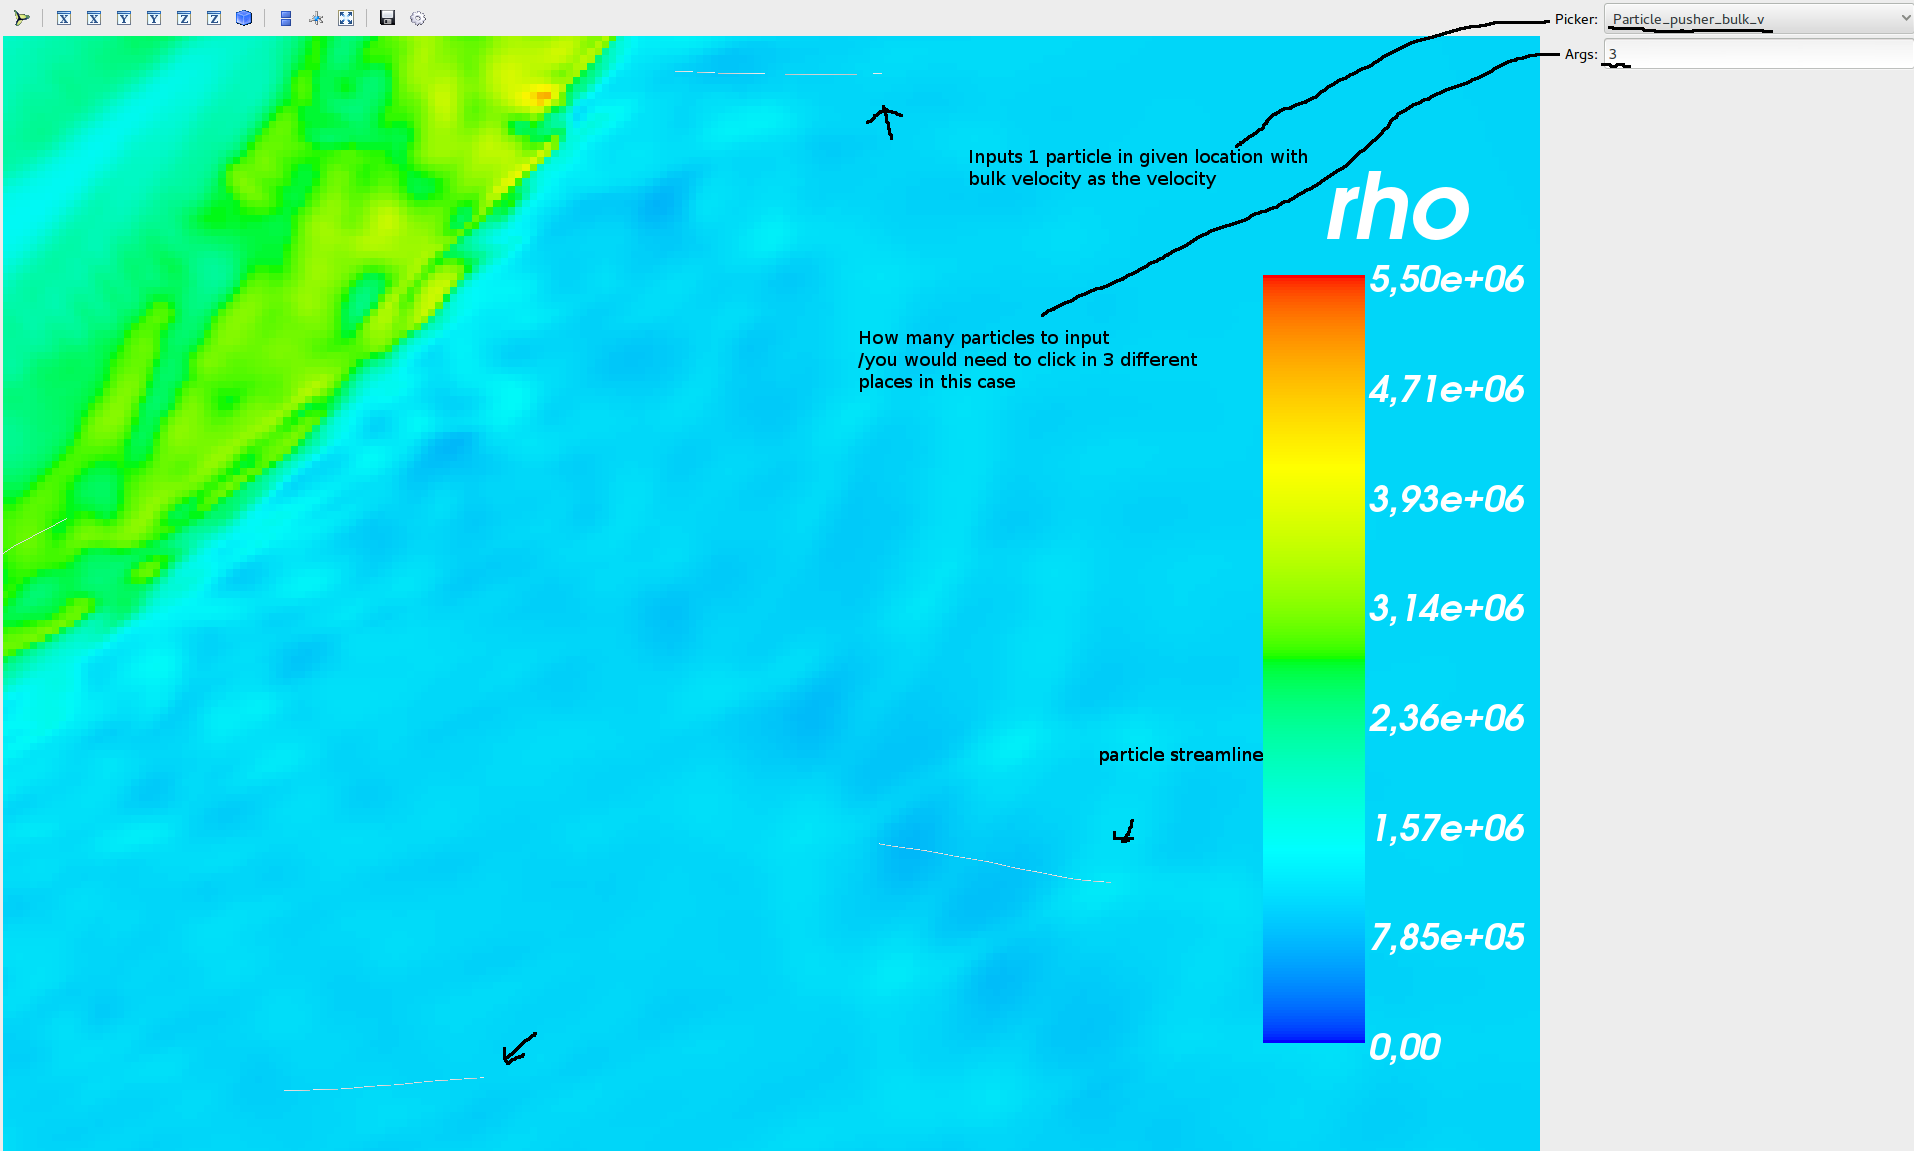
\includegraphics[width=\textwidth]{../images/particlepusherbulk.png}
 \caption{Particle pusher usage for bulk velocity sampling}
 \label{fig:particle1}
\end{figure}

\begin{figure}[H]
 \centering
 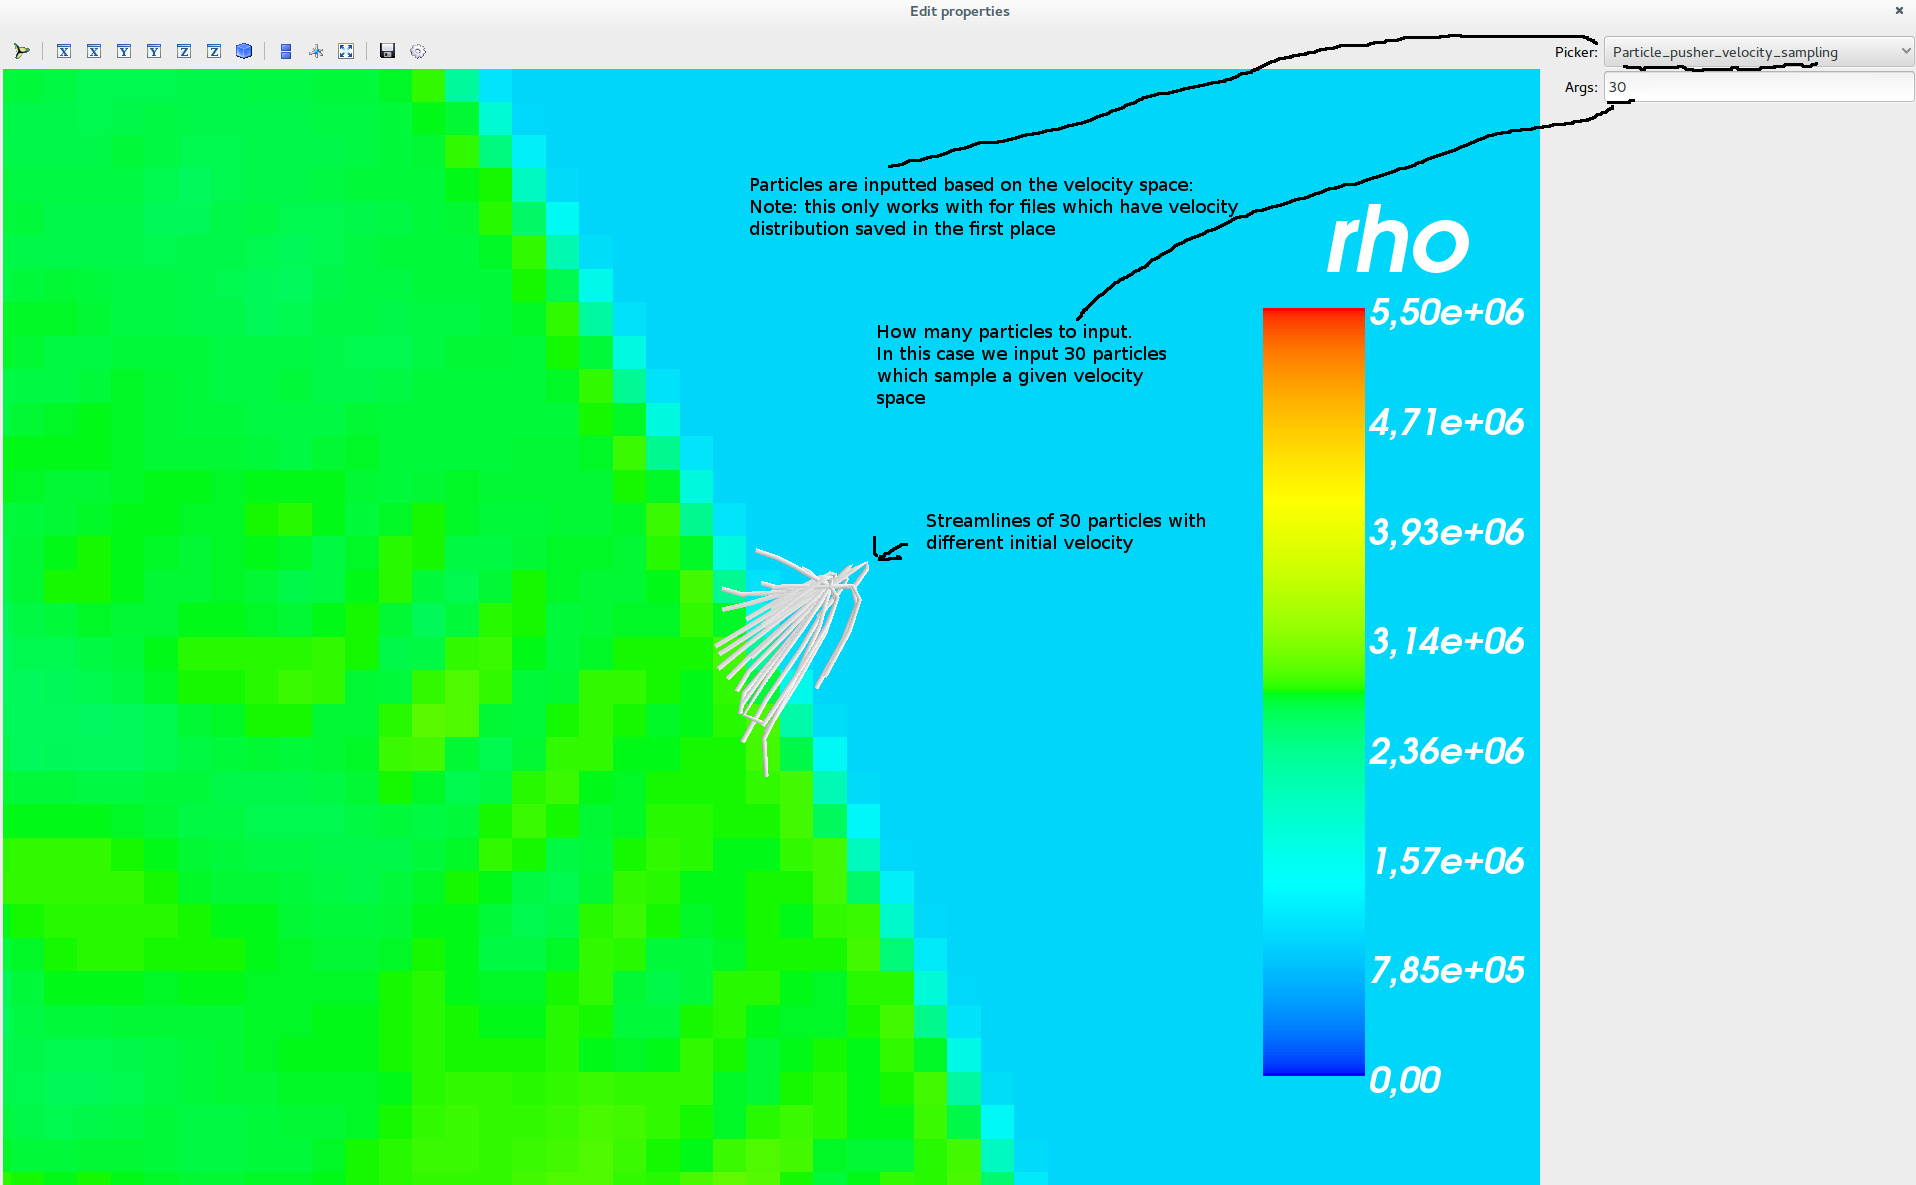
\includegraphics[width=\textwidth]{../images/particlepushersampling.png}
 \caption{Particle pusher usage for velocity space sampling}
 \label{fig:particle2}
\end{figure}


\end{document}
